\documentclass[conference]{IEEEtran}
\usepackage{times}
\usepackage[numbers]{natbib}
\usepackage{amsmath}
\usepackage{amssymb}
\usepackage{booktabs}
\usepackage{graphicx}
\usepackage{url}
\usepackage[bookmarks=true]{hyperref}

\graphicspath{ {figures/} }

\begin{document}

\title{Revisiting Pseudo-Rehearsal for Continual Learning\\with Pretrained Backbones}

\author{Dexin Huang (dh3172)\\
Columbia University\\
\texttt{dh3172@columbia.edu}}

\maketitle

\begin{abstract}
Anthony Robins's pseudo-rehearsal (Connection Science, 1995) is a
continual-learning idea that does not store data and does not train a
generator. It feeds random input vectors through the old network, treats the
outputs as pseudo-targets, and mixes those pairs into training on the new
task. The method dropped out of the literature. Generative replay and
model-inversion replay replaced it. I revisit the original recipe in the
regime that now dominates continual learning: a frozen
ImageNet-pretrained backbone with a small head trained sequentially. The
question is whether the backbone's natural-image prior makes the random
pseudo-inputs informative again. The answer is no. On Split-CIFAR-100 with a
frozen ViT-S/16 and a single 100-way linear head, the faithful Robins recipe
finishes at 0.103 final accuracy across three seeds, against 0.102 for plain
sequential fine-tuning and 0.529 for class-balanced experience replay. A
2$\times$2 ablation that swaps the input distribution (uniform random pixels
vs.\ STL-10 natural images) and the teacher source (per-task snapshot vs.\ a
joint-trained oracle head) gives the same null result in every cell.
Diagnostics show that uniform random pixels through ViT-S collapse to a
shrunken feature-space region whose dominant predicted class is exactly
$\arg\max_c (W_c \cdot \mu_{\text{random}} + b_c)$ from the joint head, but
the failure persists even when the input distribution does not collapse and
the teacher is perfect. An $\alpha$ sweep over 100$\times$ of the
distillation weight (0.5 to 50) confirms the result is not a tuning artifact:
all KD-based methods plateau between 0.10 and 0.17. The real takeaway, for
this regime, is that output-only regularization is structurally weak in
single-linear-head Class-IL with seen-class masking: in these experiments,
only class-balanced experience replay closed a meaningful fraction of the
joint-vs-sequential gap. Code:
\url{https://github.com/Dexin-Huang/pseudo-rehearsal-pretrained}.
\end{abstract}

\section{Introduction}

A neural network trained sequentially on a stream of tasks destroys what it
learned on earlier tasks. McCloskey and Cohen called this catastrophic
forgetting \citep{mccloskey1989catastrophic}, and it is still the central
problem of continual learning. Approaches split into three families:
regularization (constrain the parameters or outputs), rehearsal (keep some
old examples around and replay them), and architectural (allocate new
capacity per task). I revisit the oldest rehearsal-without-storage idea,
Robins's pseudo-rehearsal \citep{robins1995pseudorehearsal}.

The mechanics are simple. After training on task $t$, freeze a copy of the
network as a teacher. While training on task $t+1$, also sample random
inputs $r$, run them through the teacher to get pseudo-targets $q = f_t(r)$,
and mix $(r, q)$ pairs into the new-task batches. The student is nudged to
keep producing the teacher's outputs on randomly sampled inputs. There is
no stored data and no learned generator. The idea predates GANs and VAEs
and predates Shin et al.'s deep generative replay
\citep{shin2017dgr} by more than two decades.

Pseudo-rehearsal mostly dropped out of the literature. The conventional
explanation is that random inputs to a small from-scratch MLP are
off-manifold, so the teacher's response on them is uninformative about the
old decision boundary. Modern continual learning instead uses learned
generators \citep{shin2017dgr, buzzega2020der}, real-exemplar replay, or
model-inversion replay \citep{yin2020deepinversion, smith2021abd}. A
separate recent line uses frozen ImageNet-pretrained backbones with small
prompts or heads on top \citep{wang2022l2p}, where the backbone supplies
most of the representation.

That last regime is what makes the Robins revisit interesting now. The
question is narrow: in the frozen-pretrained-backbone setting, does
Robins's original recipe (uniform random pixels through the same backbone,
snapshot teacher, KD onto a small student head) recover most of the benefit
of methods that require real past data or a learned generator?

The answer here is no. I run a controlled six-method comparison plus three
diagnostic extensions on Split-CIFAR-100 with a frozen ViT-S/16 backbone
(Section~\ref{sec:method}). The Robins recipe finishes at average accuracy
0.103, within seed noise of plain sequential fine-tuning (0.102) and well
below class-balanced experience replay (0.529). A 2$\times$2 ablation over
input distribution and teacher quality plus an $\alpha$ sweep over the KD
weight leaves the negative result untouched
(Section~\ref{sec:experiments}). The mechanism check shows that ViT-S
maps uniform random pixels to a tight feature-space region whose dominant
predicted class is geometrically determined by
$\arg\max_c (W_c \cdot \mu_{\text{random}} + b_c)$. The prediction
is class 23. The empirical top class is class 23. They match exactly.

The deeper finding is sharper than the conventional dismissal. Even
non-collapsing natural inputs and an oracle teacher do not rescue
pseudo-rehearsal at any $\alpha$ tested
(Section~\ref{sec:discussion}). In this regime, output-only
regularization is weak: the methods that closed the joint-vs-sequential
gap in these experiments were the ones that put real per-example
old-class supervision into the training batch.

\section{Background}

\subsection{Pseudo-rehearsal}

Robins's procedure \citep{robins1995pseudorehearsal} snapshots the
network as a teacher $f_t$ at the end of task $t$. During task $t+1$,
each step also draws random inputs $r$ from a simple distribution (uniform
pixels in the original paper), computes pseudo-targets $q = f_t(r)$, and
adds $(r, q)$ to the batch with a distillation loss. The Connection
Science paper used a small MLP and reported some benefit on toy sequential
tasks. Atkinson et al.\ \citep{atkinson2018pseudorehearsal} extended it
to deep RL. Otherwise the line saw little modern follow-up.

\subsection{Generative and model-inversion replay}

The natural successor to Robins replaces random inputs with samples from a
model. Shin et al.\ \citep{shin2017dgr} train a GAN per task as the
generator. Later work uses VAEs or normalizing flows. Yin et al.\
\citep{yin2020deepinversion} propose DeepInversion, which inverts
classifier features to synthesize replay data. Smith et al.\
\citep{smith2021abd} extend this to continual learning as Always-Be-Dreaming.
These methods are data-free in the same sense Robins is. They also do
substantial extra work, either training a generator or running expensive
inversion every task, to produce inputs that lie on or near the data
manifold.

\subsection{Other regularization}

Elastic Weight Consolidation \citep{kirkpatrick2017ewc} penalizes
parameter drift weighted by the previous task's diagonal Fisher
information. The online variant \citep{schwarz2018onlineewc} accumulates
Fisher across tasks. Learning without Forgetting
\citep{li2017lwf} distills the previous teacher onto the current task's
real features. LwF is the closest comparator to pseudo-rehearsal. It
differs only in the input distribution used for distillation. Experience
replay stores a small buffer of past examples; the class-balanced variant
keeps a fixed number per seen class.

\subsection{Pretrained-backbone continual learning}

Recent work attaches small prompts to a frozen ImageNet-pretrained ViT and
trains those per task \citep{wang2022l2p}. The frozen backbone supplies
the representation. The per-task adaptation is small. This regime is what
makes the Robins revisit interesting now. The backbone might supply the
natural-image prior that random pseudo-inputs need.

\section{Method}\label{sec:method}

\subsection{Setting}

The dataset is Split-CIFAR-100 in 10 tasks of 10 classes each. Class
permutations are part of the seed. Each of three seeds defines an
independent grouping. Within each task there are 5{,}000 train and 1{,}000
test images.

The backbone is \texttt{vit\_small\_patch16\_224.augreg\_in21k\_ft\_in1k}
from \texttt{timm} \citep{wightman2019timm}, pretrained on ImageNet-21k
and fine-tuned on ImageNet-1k. CIFAR-100 images are upsampled to
224$\times$224 with bilinear interpolation and ImageNet-normalized. The
backbone is frozen throughout. CIFAR-100 train/test features, a 100{,}000
random-pixel pool, and a 100{,}000-sample STL-10 unlabeled pool are
precomputed once. Each ``training run'' then operates on cached
384-dimensional CLS-token features. A full 10-task continual run takes
seconds.

The head is a single linear layer \texttt{Linear(384, 100)} with bias,
about 38{,}500 parameters. The linear-head choice is deliberate. It removes
head capacity as a confound. Class-IL evaluation uses argmax over the full
100-way head, restricted to seen classes at the current point.

All cross-entropy and KD losses use additive $-\infty$ masks on
unseen-class logits. Sequential training is never asked to predict away
classes it has not yet seen as targets. Without this masking, sequential
fine-tuning would supply implicit negative gradients on future classes and
would introduce a logit-suppression artifact separate from the catastrophic
forgetting question.

\subsection{Methods compared}

All methods optimize the same linear head with AdamW (lr = $10^{-3}$, batch
256, 10 epochs per task) on cached features.

\textbf{Sequential.} Default seen-class-masked cross-entropy on
current-task data only. Lower bound.

\textbf{Joint.} The same head trained once on all 100 classes. Upper
bound.

\textbf{Class-balanced replay.} Buffer of 5 examples per seen class, up
to 500 total. Each training batch is half current-task and half buffer at
constant total batch size.

\textbf{Online EWC.} Diagonal empirical Fisher computed in closed form for
a masked linear-CE head:
\begin{equation}
F_W[c, j] = \frac{1}{N} \sum_i (p_i[c] - \mathbb{1}\{c = y_i\})^2 \cdot x_i[j]^2.
\end{equation}
Fisher is accumulated across tasks. One running $\theta^*$ is kept.

\textbf{Pseudo-rehearsal (Robins, faithful).} At the start of task $t+1$,
snapshot the head as teacher $h_t$. Per step, sample $\text{batch\_size}$
random images (pixels uniform $[0, 1]$, ImageNet-normalized), pass them
through the frozen ViT (cached in advance), run the teacher, restrict to
previously-seen classes (seen minus current), and add $\alpha \cdot
\text{KD}(q_{\text{old}}, p_{\text{student}})$ where KD is soft-label
cross-entropy in teacher-to-student direction. Default $\alpha = 1.0$.

\textbf{LwF.} Same KD machinery as pseudo-rehearsal but the distillation
inputs are the current-task real features
\citep{li2017lwf}.

\subsection{2$\times$2 ablation and $\alpha$ sweep}

The first sweep (six methods, three seeds, 18 runs) returns a clean null
for pseudo-rehearsal. Two natural rescue stories follow. Each is tested
independently.

The first replaces uniform random pixels with STL-10 unlabeled features
through the same ViT (\texttt{pseudo\_natural}). STL-10 is 100{,}000 real
natural images, out-of-distribution for CIFAR-100. If pseudo-rehearsal
needs natural-image structure in the inputs rather than random noise, this
should help.

The second replaces the snapshot teacher with the joint-trained head loaded
from a checkpoint (\texttt{pseudo\_oracle}). This is information leakage.
The oracle has seen all 100 classes. It is not a valid method, only a
diagnostic. If pseudo-rehearsal fails because the snapshot teacher
accumulates errors during CL, an oracle teacher should rescue it.

The third combines both (\texttt{pseudo\_oracle\_natural}), giving the
best-case for pseudo-rehearsal across the two factors. The second sweep
adds 3 new pseudo variants $\times$ 3 seeds $=$ 9 runs.

A third sweep addresses the tuning critique. It varies the KD weight
$\alpha \in \{0.5, 1, 5, 10, 50\}$ on \texttt{pseudo},
\texttt{pseudo\_oracle}, and \texttt{lwf} (45 runs). At sufficiently large
$\alpha$ the KD term dominates the new-task CE term. The student must mimic
the teacher. For \texttt{pseudo\_oracle} this should in principle approach
joint accuracy. The question is how the curve looks in between.

\subsection{Mechanism check}

The diagnostic story for pseudo-rehearsal's failure should not lean on
hand-waving about ``off-manifold inputs.'' I make a sharp prediction. The
dominant pseudo-target class on random inputs is determined by the
geometry of the (random-feature mean, joint head) pair alone:
\begin{equation}
\hat{c} = \arg\max_c \bigl( W_c \cdot \mu_{\text{random}} + b_c \bigr).
\label{eq:mechanism}
\end{equation}
If random features collapse tightly enough (small per-dimension standard
deviation around the mean), per-sample variation is negligible. The
head's response on the mean random feature predicts the dominant argmax.
$\mu_{\text{random}}$ is computed over the 100{,}000-sample random pool.
$\hat{c}$ is compared against the empirical top class.

\subsection{Diagnostic probes}

To characterize how random pixels through ViT land in feature space, I
report (i) $L_2$ norm mean and standard deviation of real vs.\ random
features, (ii) nearest-neighbor cosine distance from a 5K random sample to
a 5K real sample, (iii) predictive entropy of the joint head on real vs.\
random features, and (iv) the top-class histogram of joint-head predictions
over the 100{,}000-sample random pool.

\section{Experiments}\label{sec:experiments}

\subsection{Main comparison}

Final accuracy on Split-CIFAR-100, mean $\pm$ std over three seeds, is
shown in Table~\ref{tab:main}. The 2$\times$2 ablation view is in
Table~\ref{tab:twobytwo}. The running-average accuracy and final per-task
accuracy plots are in Fig.~\ref{fig:curves}.

\begin{table}[t]
\centering
\caption{Final accuracy, forgetting (FGT), and backward transfer (BWT) on
Split-CIFAR-100 with a frozen ViT-S/16 and a 100-way linear head, three
seeds. FGT and $-$BWT match because the per-task argmax happens at the
diagonal.}
\label{tab:main}
\small
\begin{tabular}{@{}lrrr@{}}
\toprule
Method & ACC & FGT & BWT \\
\midrule
Joint (UB)              & \textbf{0.788} $\pm$ 0.000 & 0.000 & n/a \\
Replay (5/class)        & \textbf{0.529} $\pm$ 0.004 & 0.450 & $-$0.450 \\
EWC (online)            & 0.192 $\pm$ 0.010 & 0.825 & $-$0.825 \\
LwF                     & 0.111 $\pm$ 0.012 & 0.919 & $-$0.919 \\
Pseudo-natural          & 0.106 $\pm$ 0.008 & 0.923 & $-$0.923 \\
Pseudo-oracle           & 0.105 $\pm$ 0.005 & 0.925 & $-$0.925 \\
Pseudo (Robins)         & 0.103 $\pm$ 0.005 & 0.927 & $-$0.927 \\
Sequential (LB)         & 0.102 $\pm$ 0.004 & 0.928 & $-$0.928 \\
Pseudo-oracle-natural   & 0.099 $\pm$ 0.003 & 0.932 & $-$0.932 \\
\bottomrule
\end{tabular}
\end{table}

\begin{table}[t]
\centering
\caption{2$\times$2 ablation over the two pseudo-rehearsal factors. All
four cells overlap within seed noise.}
\label{tab:twobytwo}
\small
\begin{tabular}{@{}lcc@{}}
\toprule
Teacher source & Random pixels & STL-10 natural \\
\midrule
CL snapshot        & 0.103 & 0.106 \\
Joint (oracle)     & 0.105 & 0.099 \\
\bottomrule
\end{tabular}
\end{table}

All four pseudo cells overlap within seed noise. Switching the input
distribution from random pixels to STL-10 natural images does not help.
Replacing the snapshot teacher with the joint-trained oracle does not
help. LwF lands in the same neighborhood. EWC offers a modest gain. It
constrains the linear head's drift but cannot supply the missing per-class
signal. Only class-balanced experience replay separates from the bottom
group. At 0.529 it reaches about two-thirds of the joint upper bound
while storing 500 features total.

\subsection{$\alpha$ sweep}

Sweeping the KD weight $\alpha$ over two orders of magnitude
(Fig.~\ref{fig:alpha}, Table~\ref{tab:alpha}) shows the failure is not a
tuning artifact. All three KD methods trace nearly parallel monotonic
curves. The oracle teacher provides no meaningful advantage over the
snapshot teacher at any $\alpha$ tested. At $\alpha \to \infty$ the KD term
would dominate CE and the student would converge to the teacher,
recovering joint accuracy for \texttt{pseudo\_oracle}. In the explored
range the curve has not begun to bend toward that limit. Even at
$\alpha = 50$ the gain over the default $\alpha = 1$ is only 0.04 to 0.05.

\begin{table}[t]
\centering
\caption{$\alpha$ sweep on KD methods, three seeds each. All three methods
gain less than 0.06 across two orders of magnitude.}
\label{tab:alpha}
\small
\begin{tabular}{@{}lrrrrr@{}}
\toprule
& $\alpha {=} 0.5$ & $\alpha {=} 1$ & $\alpha {=} 5$ & $\alpha {=} 10$ & $\alpha {=} 50$ \\
\midrule
LwF             & 0.110 & 0.111 & 0.114 & 0.117 & 0.164 \\
Pseudo          & 0.103 & 0.103 & 0.107 & 0.114 & 0.144 \\
Pseudo-oracle   & 0.103 & 0.105 & 0.111 & 0.118 & 0.142 \\
\bottomrule
\end{tabular}
\end{table}

\begin{figure}[t]
\centering
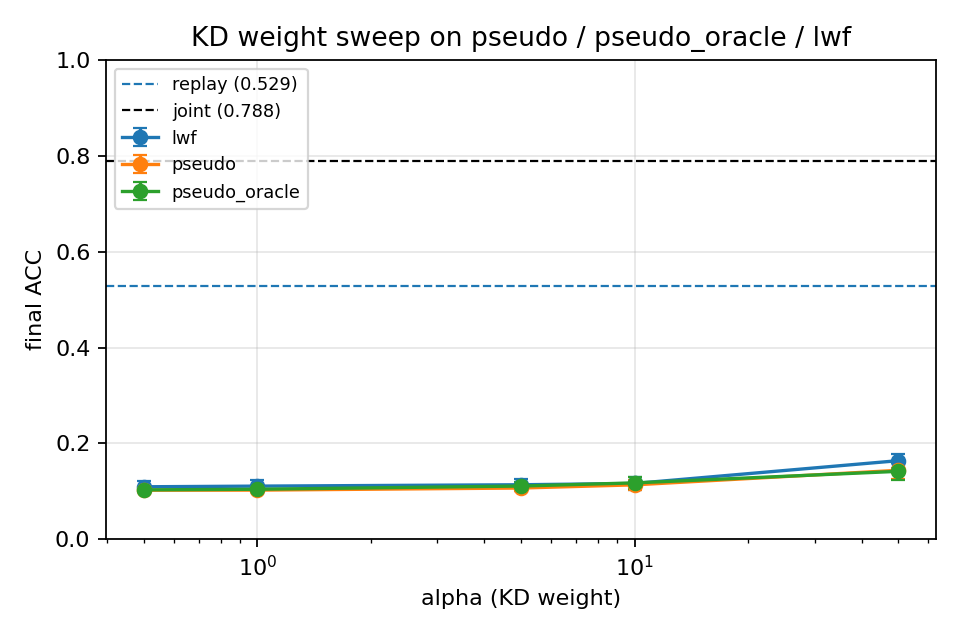
\includegraphics[width=\linewidth]{alpha_sweep.png}
\caption{KD weight sweep on the three distillation methods.
Log $x$-axis. Replay (dashed blue, 0.529) and joint (dashed black, 0.788)
are reference lines. All three KD curves crawl from 0.10 to 0.16 across
two orders of magnitude. The oracle teacher offers no consistent
advantage.}
\label{fig:alpha}
\end{figure}

\begin{figure}[t]
\centering
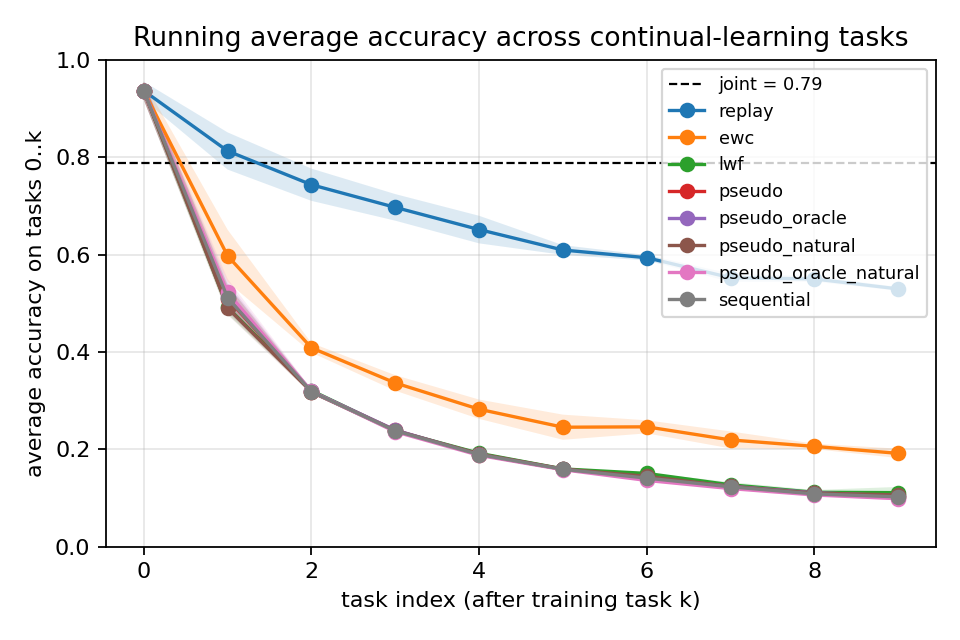
\includegraphics[width=\linewidth]{running_avg_accuracy.png}
\caption{Running mean accuracy across continual-learning tasks. Replay
separates from the pack immediately and decays gracefully. EWC tracks
slightly above the bottom group. The four pseudo variants, LwF, and
sequential are visually indistinguishable across all 10 tasks.}
\label{fig:curves}
\end{figure}

\subsection{Diagnostics}

Diagnostics use the joint head from seed 0 as a fixed teacher on the
100{,}000-sample random pool. Real-feature $L_2$ norm is
49.52 $\pm$ 1.70. Random-feature $L_2$ norm is 34.33 $\pm$ 1.77.
Random features sit in a sphere about 31\% smaller in radius. Mean
nearest-neighbor cosine of random to real is 0.392
(p25 0.381, p75 0.401). Real CIFAR features are far from random-pixel
features in direction.

Predictive entropy on real features is 0.513 nats. On random features it
is 2.666 nats. Uniform-over-100 reference is 4.605 nats. The teacher is
more uncertain on random inputs but not uniformly so. The top-class
histogram tells the rest of the story. Class 23 takes 62.7\% of all argmax
predictions on the random pool. The teacher predicts only 4 of 100 classes
anywhere across the 100{,}000 random inputs. Distribution entropy over
predicted classes is 0.664 nats.

\subsection{Mechanism check}

The geometric prediction in Eq.~\ref{eq:mechanism} holds exactly.
$\arg\max_c (W_c \cdot \mu_{\text{random}} + b_c) = 23$. The empirical top
class on the random pool is 23. The top-3 predicted classes from the mean
feature are $\{23, 60, 76\}$. Class 23 dominates. The per-dimension
standard deviation of the random pool, averaged across 384 dimensions, is
0.305. The random-feature distribution is tight enough that per-sample
variation does not change the argmax. The random-pixel collapse is fully
determined by the joint head and the mean random feature.

\section{Discussion}\label{sec:discussion}

\subsection{The mechanism story is sharper than the conventional one}

The standard dismissal of Robins is that random inputs are off-manifold and
the teacher is uninformative on them. The diagnostics confirm this. Random
pixels through ViT-S land in a tight shrunken region of feature space. The
teacher classifies 62.7\% of them as one dominant class. The mechanism
check goes further. The collapse is geometrically predictable from the
mean random feature and the head's weights. Robins's recipe at the unit of
analysis was always going to give the student degenerate pseudo-soft-targets,
a near-constant signal pointing at one arbitrary class.

\subsection{The conventional story is not the whole story}

The 2$\times$2 ablation eliminates two natural rescue stories. STL-10
images are real natural images and produce non-degenerate teacher
distributions on this backbone. They do not move the result. The oracle
teacher, the joint classifier with full knowledge of all 100 classes,
also does not move it. Both factors combined still fail. The off-manifold
collapse alone is not the full diagnosis, at least under this input
choice and this optimization budget. STL-10 is a single out-of-distribution
natural-image source, not a guarantee that no natural-image distribution
could help; an exhaustive input-distribution sweep is left to future
work.

\subsection{A more local diagnosis}

In single-linear-head Class-IL with seen-class masking, every training step
on task $t$ supplies per-class cross-entropy gradients on 5{,}000 fresh
examples per epoch. The head is aggressively rewritten toward the current
task's 10 classes. KD on previously-seen classes adds a counter-pressure
on the old-class logits. It acts only through the outputs, not through the
per-example supervision the new task gets. Even at $\alpha = 50$ the KD
term does not match the CE term's gradient mass without effectively
shutting down new-task learning. This generalizes a known observation
about LwF's weakness in Class-IL, where the head develops a recency bias.
The extension here is that the weakness survives the rescue stories
tested: a different input distribution and a perfect teacher.

Replay works for the symmetric reason. It injects real per-example
old-class supervision into the batch, on the same footing as new-task
examples. EWC partially works because it constrains the head's weights
from drifting at all, an approach independent of class-level signal.
Output-only regularization in this regime sits between the two: it
neither freezes the parameters nor supplies per-example old-class
gradient.

\subsection{Connection to data-free continual learning}

The finding sharpens what data-free CL needs. DeepInversion
\citep{yin2020deepinversion} and ABD \citep{smith2021abd} are both
data-free in Robins's sense. They also do substantial extra work to
produce inputs that lie on the data manifold and elicit class-discriminative
responses from the teacher. The implicit assumption is that the input
distribution is what was missing from Robins. This paper suggests that, at
least in the linear-head Class-IL regime, the input distribution is not
the bottleneck. The structural separation between output-only and
example-level supervision is. Whether the same holds when the backbone is
fine-tunable, or when the head has more capacity, is left to future work.

\subsection{Limitations}

The paper studies one backbone (ViT-S/16, ImageNet-21k $\to$ 1k), one
dataset (Split-CIFAR-100), one continual setting (Class-IL, 10 tasks
$\times$ 10 classes), one head (linear), one feature-precomputation regime
(frozen backbone), three seeds, and one out-of-distribution natural-image
source (STL-10). A CLIP or DINO backbone could place random features in a
different feature-space region. A multi-layer MLP head or a fine-tunable
backbone introduces representational degrees of freedom that EWC and LwF
were originally designed to protect. The $\alpha$ sweep stops at 50. At
$\alpha \to \infty$ \texttt{pseudo\_oracle} approaches joint accuracy by
abandoning new-task learning, but only under the assumption that KD on
the chosen pseudo-input distribution identifies the joint head's
old-class decision boundary; output matching on off-manifold features
need not constrain CIFAR class boundaries even in the limit. The replay
number depends on storing 5 examples per class, small but not zero. A
fair no-storage floor for pseudo-rehearsal is plain sequential FT, which
is what it matches. The paper does not include a class-mean / prototype
replay comparator (one stored vector per seen class, no per-example
exemplars). Such a comparator would sharpen the distinction the
discussion draws between output-only regularization and example-level
supervision; it is the most direct experimental follow-up.

\section{Conclusion}

The question was whether a frozen ImageNet-pretrained backbone makes
Robins's 1995 pseudo-rehearsal competitive again, in the regime where
that question is most natural. The answer here is no, across three
rescue stories: a single natural-image input source (STL-10), an oracle
teacher, and a 100$\times$ sweep of the KD weight. The random-pixel
collapse in feature space is real and geometrically predictable, but it
is not the only obstacle: STL-10 inputs and an oracle teacher do not
move the number either. In this regime, output-only regularization is
weak compared to methods that put per-example old-class supervision in
the batch. The cheapest competitive method in these experiments stores 5
features per seen class.

\section*{Code and Reproducibility}

All code, configs, cached features, and result JSON files are at
\url{https://github.com/Dexin-Huang/pseudo-rehearsal-pretrained}. The
reported numbers come from 72 training runs (six baseline methods, three
extension methods, $\alpha$ sweep on three methods $\times$ five
$\alpha$ values), three seeds each, on RTX 4090 secure-cloud pods. Total
compute was under one hour of GPU time. Mean-aggregation and FGT/BWT
formulas are in \texttt{evaluate.py}. The mechanism check is in
\texttt{mechanism\_check.py}. Plots are in \texttt{plots.py} and
\texttt{analyze\_alpha.py}.

\clearpage

\bibliographystyle{plainnat}
\bibliography{references}

\end{document}
